\documentclass{report}

% Layout
\usepackage[a4paper, margin=1.5in]{geometry}
\usepackage{parskip}

\usepackage{amsmath}
\usepackage{amssymb}
\usepackage{amsthm}
\usepackage{graphicx}
\usepackage{caption}
\usepackage{subcaption}
\usepackage{tabularx}
\usepackage{xcolor}
\usepackage{float}

% Fonts
\usepackage{pxfonts}

% Colors
\definecolor{pink}{rgb}{0.780,0.223,0.537}
\definecolor{reddish}{rgb}{0.769,0.263,0.169}
\definecolor{darkblue}{rgb}{0.012,0.184,0.384}
\definecolor{blue}{rgb}{0.000,0.361,0.773}
\definecolor{purple}{rgb}{0.435,0.259,0.757}
\definecolor{orange}{rgb}{0.890,0.384,0.035}
\definecolor{green}{rgb}{0.102,0.498,0.216}
\definecolor{red}{rgb}{0.812,0.133,0.180}

% References
\usepackage{hyperref}
\hypersetup{
  colorlinks,
  linkcolor=blue,
  citecolor=blue
}
\renewcommand{\UrlFont}{\color{purple}\ttfamily}

% Bibliography and citation style
\usepackage[square]{natbib}
\bibliographystyle{apalike}
\renewcommand{\refname}{Bibliography}

% Code listings
\usepackage{listings}
\lstset{
  breaklines=true,
  frame=lines,
  captionpos=b,
  belowskip=0pt,
  basicstyle=\ttfamily,
  stringstyle=\color{blue},
  keywordstyle=\color{reddish},
  commentstyle=\color{green}
}
\lstdefinelanguage{Cypher}{
  language=SQL,
  morekeywords={RETURN,FOR,REQUIRE,IS,WITH,CALL,YIELD}
}
\lstdefinelanguage{GSQL}{
  language=SQL,
  morekeywords={VERTEX,EDGE,DIRECTED,PRIMARY_ID,TO,ACCUM,PRINT},
  deletekeywords={ROLE}
}

% Definitions
\theoremstyle{definition}
\newtheorem{definition}{Definition}
\newcommand{\definitionautorefname}{Definition}

% Natural numbers
\newcommand{\N}{\mathbb{N}}

% Partial function
\makeatletter
\newcommand{\pto}{}% just for safety
\DeclareRobustCommand{\pto}{\mathrel{\mathpalette\p@to@gets\to}}
\newcommand{\p@to@gets}[2]{%
  \ooalign{\hidewidth$\m@th#1\mapstochar\mkern5mu$\hidewidth\cr$\m@th#1\to$\cr}%
}
\makeatother

% Source and target operators
\newcommand{\src}{\mathtt{src}}
\newcommand{\trg}{\mathtt{trg}}

% Schema elements
\newcommand{\ptype}{\tau}
\newcommand{\ptypes}{\mathcal{T}}
\newcommand{\rtype}{\tau^\mathsf{r}}
\newcommand{\rtypes}{\mathcal{T}^\mathsf{r}}
\newcommand{\otype}{\tau^\mathsf{o}}
\newcommand{\otypes}{\mathcal{T}^\mathsf{o}}

% Semantics (double brackets)
\newcommand{\lsem}{\ensuremath{[\![}}
\newcommand{\rsem}{\ensuremath{]\!]}}
\newcommand{\sem}[1]{\ensuremath{\lsem #1 \rsem}}

% Conformance relation
\newcommand{\conf}{\sqsubseteq}

% Undefined
\newcommand{\undefined}{\mathbf{undef}}

% Yes/No
\newcommand{\yes}{\color{green}\checkmark}
\newcommand{\no}{\color{red}$\times$}

\renewcommand{\itemautorefname}{Rule}

\title{Property Graph Schemas}
\author{Nimo Beeren}


\begin{document}

\maketitle

\renewcommand{\thepage}{\roman{page}}

\tableofcontents
\listoffigures
\listoftables
% TODO: use short captions for list of figures/tables

\setcounter{page}{0}
\renewcommand{\thepage}{\arabic{page}}

\chapter{Introduction}

Graph databases have been steadily growing in popularity in recent years, receiving attention in the form of fundamental research as well as practical usage. One of the spearpoints of the graph database is its flexibility. While the traditionally dominant relational data model organizes data into tables and requires a fixed schema, graphs offer a simple yet powerful model consisting of nodes and edges which can be structured freely.

However, this freedom comes at a cost. Without a schema, we miss out on opportunities for query optimization \citep{chakravarthy1990logic, buneman1997adding, meier2013semantic}, we risk degradation of data integrity, and we lack a formally verifiable source of documentation. By bringing back schemas to the graph world, the flexibility of graph databases can be combined with the robustness of relational databases.

The \emph{property graph model} is the predominant data model among graph database systems today. It provides an intuitive way of modeling entities as nodes, and their relationships as edges. Both nodes and edges are associated with labels, and they hold data in the form of key--value pairs known as \emph{properties}. We can imagine local constraints, such as mandatory properties on nodes or edges, as well as constraints on the structure of the graph, such as mandatory edges between nodes. To the best of our knowledge, there exists no published work that addresses the specification and validation of all these kinds of constraints using a single schema formalism.

Our overarching goal is to develop an end-to-end framework for property graph schema specification and validation. To this end, we propose a schema formalism capable of expressing local and structural constraints, we provide a prototypical implementation for schema validation in the form of graph queries, and we investigate the practical feasibility of this approach on current graph database systems and realistic datasets.

\chapter{Related Work}

\section{Graph Integrity Constraints}

% TODO: refer to querying graphs book instead of discussing integrity constraints here

The problem of expressing and validating integrity constraints for graphs has received some attention in the scientific community. A large part of this research has been on functional dependencies, which has been studied extensively in the context of relational databases \citep{fagin1984theory,abiteboul1999data}. The idea of functional dependencies has been adapted to graph data, with the first work focussing on \emph{key constraints}, which aim to uniquely identify entities represented by nodes \citep{fan2015keys}. These have been extended to include more general dependencies \citep{fan2016functional}. The current state of the art of key constraints is presented in \textsc{PG-Keys} \citep{angles2021keys}.

% TODO: other kinds of graph integrity constraints (pokorny 2017?)

\section{Graph Schema}

Some approaches to graph schema have been discussed in the literature. While these methods are based on different graph models, they may be adapted to the property graph model. \citet{buneman1997adding} propose a method that represents both data and schema as edge-labeled graphs. This enables the specification of the types of edges and paths that are allowed to occur in a database instance, but does not cover mandatory edges or more general cardinality constraints.

\citet{colazzo2015typing} introduce another schema formalism for edge-labeled data graphs. They define a schema as a set of pairs $(r_{in}, r_{out})$, where $r_{in}$ and $r_{out}$ are regular expressions. The semantics is that every node must match a schema element $(r_{in}, r_{out})$, meaning that the node's incoming edges match $r_{in}$ and its outgoing edges match $r_{out}$. Using Regular Path Queries (RPQs), edge cardinality can be exactly specified. When extending the language to Nested Regular Expressions (NREs), it is possible to specify structural constraints over arbitrarily large graph patterns.

SHACL\footnote{\url{https://www.w3.org/TR/shacl/}} is a language for specifying constraints on RDF graphs \citep{pan2009rdf}. These constraints themselves are also represented as RDF graphs, and are called \emph{shapes}. Constraints on values, data types and cardinality are supported. This enables specification of allowed, optional, and mandatory edges. A review of the formal frameworks used to study the SHACL language and the validation of RDF graphs against SHACL schemas can be found in \citet{pareti2022shacl}.

\section{Property Graph Schema}

The property graph data model has been adopted by numerous contemporary graph database systems (dating back to at least 2007 with the first release of Neo4j\footnote{\url{https://neo4j.com/open-source-project/}}), but a formal specification was missing until one was proposed by \citet{angles2018property}. The author also brought integrity constraints to the property graph model, and defined a basic notion of schema using first-order logic rules. In this work, no distinction was made between mandatory and optional properties, nor were cardinality constraints addressed.

\citet{bonifati2019schema} present a property graph schema validation approach based on graph homomorphisms. They differentiate between mandatory and optional properties, though edges are always interpreted as optional. Cardinality constraints are not discussed. The authors look at schemas from two different angles: they can be descriptive in the sense that they only reflect the data, or they can be prescriptive by means of enforcing constraints on data. This distinction is relevant in particular to the topic of schema evolution, where it may be desirable to switch between these two modes as an application matures. It is noted that most contemporary graph database systems only provide descriptive schema tools.

\citet{lbath2021inference} look at property graph schemas from the perspective of schema inference. Their goal is to extract an accurate and complete schema for an arbitrary property graph instance. To this end, a property graph schema formalism is defined, supporting cardinality constraints, mandatory and optional edges, as well as subtyping. In addition, a syntax for schema definition is presented, and the schema inference pipeline is evaluated using real-world datasets. The problem of validating a graph against a given schema is not addressed. Statistical methods are applied in \citep{bonifati2022hierarchical} to improve performance.

\citet{lei2021thesis} proposes a semi-automated method for schema extraction which incorporates expert knowledge. The user can adjust parameters and similarity measures which affect how the schema is generated. An implementation and experimental results are given. Cardinality constraints are not covered.

Many commercially available property graph database systems currently support some form of schema or constraints. Some require the user to specify a schema, while others infer a schema from data. We further analyze the schema capabilities of existing systems in \autoref{sec:sota}.

\chapter{Property Graphs}

We start by introducing our data model, which is based on the definition of \emph{property graph} established by the Working Group for Database Languages~(WG3) as part of ISO/IEC JTC1/SC32 \citep{deutsch2021gpml}. We use this data model in the rest of this document.

Our notion of property graph represents data as a directed attributed multigraph. Nodes and edges carry data in the form of a set of labels and a set of key--value pairs, called \emph{properties}. We use the umbrella term \emph{objects} to refer to nodes and edges. Being a \emph{multigraph}, a property graph allows the existence of multiple edges between two nodes $u$ and $v$. Furthermore, we allow $u = v$, in which case the edge is called a \emph{self-loop}. For ease of notation, we do not consider undirected edges, although they could be simulated by attaching a special label or property to an edge.

An example of a property graph is given in \autoref{fig:pg}. Nodes are drawn as boxes, and edges are drawn as arrows. Node labels are written in the top compartment, and node properties are written in the bottom compartment. Edge labels are written inside a pill and edge properties are surrounded by `\{' and `\}', which may be omitted when an edge has no properties.

For a formal definition, we assume the existence of the following countably infinite sets: the set of labels $\mathcal{L}$, the set of property names $\mathcal{N}$ and the set of property values $\mathcal{V}$.

\begin{definition}[Basic record]
  \label{def:record-basic}
  A \emph{record} is a finite partial function $r : \mathcal{N} \pto \mathcal{V}$ that maps some property names to property values. The set of all records is denoted as $\mathcal{R}$.
\end{definition}

\begin{definition}[Property graph]
  \label{def:pg}
  A \emph{property graph} is a tuple $$G = (N, E, \rho, \lambda, \pi)$$ where
  \begin{itemize}
    \item $N$ is a finite set of nodes;
    \item $E$ is a finite set of edges such that $N \cap E = \emptyset$;
    \item $\rho : E \to (N \times N)$ is a total function mapping edges to ordered pairs of nodes;
    \item $\lambda : (N \cup E) \to 2^{\mathcal{L}}$ is a total function mapping nodes and edges to a (possibly empty) set of labels;
    \item $\pi : (N \cup E) \to \mathcal{R}$ is a total function mapping nodes and edges to a record.
  \end{itemize}
\end{definition}

Given a node $u$, the set of \emph{outgoing} edges is given by $\{e \in E \mid \exists v \in N : \rho(e) = (u, v)\}$, and the set of \emph{incoming} edges is given by $\{e \in E \mid \exists v \in N : \rho(e) = (v, u)\}$.

The functions $\src$ and $\trg$ map pairs to their first and second element, i.e. $\src((u, v)) = u$ and $\trg((u, v)) = v$. To refer to the source and target \emph{endpoints} of an edge $e$, we may write $\src(\rho(e))$ and $\trg(\rho(e))$ respectively.

\begin{figure}[t]
  \centering
  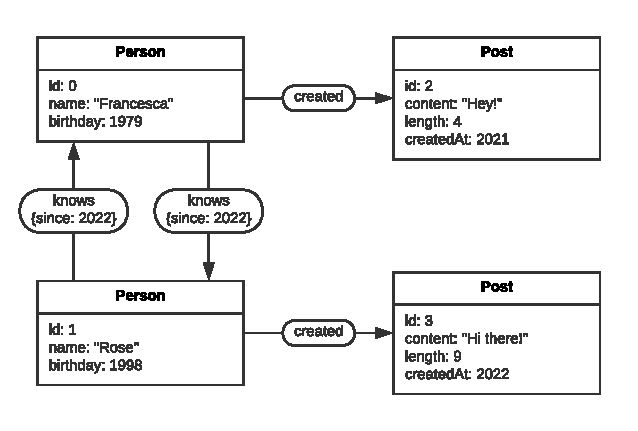
\includegraphics{figures/pg.pdf}
  \caption{A property graph representing a small social network.}
  \label{fig:pg}
\end{figure}

\chapter{Property Graph Schemas}

A schema should allow modeling of real-world entities and their relationships. A more expressive schema language enables the specification of more complex constraints, but may come at a cost of greater research and engineering effort, as well as worse runtime performance. This needs to be balanced in our choice of schema language.

To explore the schema features that are commonly used in practice, let us look at some existing data modeling techniques. As a baseline, we consider the Entity--Relationship (ER) model as proposed by~\citet{chen1976entity}. This model incorporates entities, relationships, attributes, and values. An \emph{entity} is a ``thing'' that can be uniquely identified, a \emph{relationship} is an association between entities, and an \emph{attribute--value} pair represents information about an entity or relationship. Furthermore, an entity may have a \emph{role} in a relationship, such as ``wife'' or ``husband'' in a marriage relationship. These are the concepts underlying many conceptual data modeling methods in use today.

After the original specification, the ER model has been extended in various ways. For example, a notation which introduced cardinality constraints, optionality, and subtype relations was developed by~\citet{barker1990entity}. With these additions, we can create a more nuanced data model which fits the real world more closely.

In the next subsection, we first establish a basic definition of property graph schema, which we then extend with additional features such as cardinality constraints (\autoref{sec:cardinality}) and optional properties (\autoref{sec:optional-properties}).

\section{Basic definition}

In this subsection, we define a notion of property graph schema which incorporates the basic features of the ER model: entities, relationships, attributes, and values.

\autoref{tab:er-pg} shows how the basic elements of the ER model can be mapped to the property graph model. Note that there are no named roles in the property graph model, but the direction of an edge does allow the distinction between the source and target of an edge. Conversely, the direction of an edge can be represented using roles in the ER model.

\begin{table}[t]
  \centering
  \begin{tabular}{|l|l|}
    \hline
    \textbf{ER}  & \textbf{PG}     \\
    \hline
    Entity       & Node            \\
    Relationship & Edge            \\
    Attribute    & Property name   \\
    Value        & Value           \\
    Role         & Edge direction* \\
    \hline
  \end{tabular}
  \caption{Mapping between entity--relationship and property graph concepts. Roles and edge direction can be used for similar purposes, but are not equivalent.}
  \label{tab:er-pg}
\end{table}

An example of a basic property graph schema is given in \autoref{fig:pg-schema-basic}. The similarity between property graphs and schemas allows us to visualize and think about them using the same mental model. Schema nodes and edges are drawn in the same way as for data graphs, but properties are associated with types rather than concrete values.

\begin{figure}[t]
  \centering
  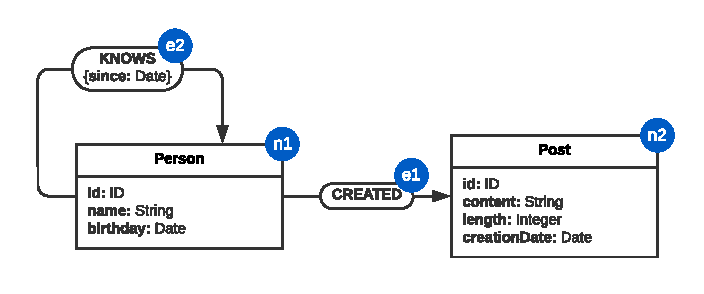
\includegraphics{figures/pg-schema-basic.pdf}
  \caption{A basic property graph schema.}
  \label{fig:pg-schema-basic}
\end{figure}

To formally define property graph schemas and schema conformance, we first assume the existence of a set of property types $\mathcal{T}$. Next, we introduce a number of supporting concepts.

\begin{definition}[Basic property conformance]
  \label{def:property-conformance-basic}
  For each property type $\ptype \in \ptypes$ there is a set $\sem{\ptype} \subseteq \mathcal{V}$ that contains all property values that \emph{conform} to the type $\ptype$.
\end{definition}

The concept of property type is similar to a \emph{value set} in the ER model. Value sets and property types are used to specify which values may be associated with an attribute, or which values a property is allowed to have\footnote{Note the subtle difference in terminology: an ER attribute is associated with a value, whereas a property has a name and a value}. A minor difference is that \citet{chen1976entity} postulates that values from different value sets can be equivalent, while we do not have a notion of value equivalence.

\begin{definition}[Basic record type]
  \label{def:record-type-basic}
  A \emph{record type} is a finite partial function $\rtype : \mathcal{N} \pto \ptypes$ that maps some property names to a property type.
  % We denote such record types as $\langle a_1 : \ptype_1, \ldots, a_n : \ptype_n \rangle$.
\end{definition}

\begin{definition}[Basic record conformance]
  \label{def:record-conformance-basic}
  We say that a record $r$ \emph{conforms} to a record type $\rtype$, denoted $r \in \sem{\rtype}$, if for each property name $k \in \mathcal{N}$ it holds that (1) $r(k)$ is defined iff $\rtype(k)$ is defined and (2) $r(k) \in \sem{\rtype(k)}$ if $r(k)$ and $\rtype(k)$ are defined.
\end{definition}

\begin{definition}[Object type]
  \label{def:object-type}
  An \emph{object type} is a pair $\otype = (L, \rtype)$ where $L \subseteq \mathcal{L}$ is a finite set of labels and and $\rtype$ a record type.
  % We denote such object types also simply as $L\rtype$ or $\{ l_1 \ldots l_k \} \langle a_1 : \rtype_1, \ldots, a_n : \rtype_n \rangle$.
  The set of all object types is denoted as $\otypes$.
\end{definition}

\begin{definition}[Object conformance]
  \label{def:object-conformance}
  Let $G = (N, E, \rho, \lambda, \pi)$ be a property graph and $\otype = (L, \rtype)$ an object type. The set of objects that \emph{conform} to $\otype$ is defined as $\sem{\otype} = \{o \in N \cup E \mid \lambda(o) = L \wedge \pi(o) \in \sem{\rtype}\}$.
\end{definition}

\begin{definition}[Basic property graph schema]
  \label{def:pg-schema-basic}
  A \emph{property graph schema} is a tuple $$S = (N, E, \rho, \omega)$$ where
  \begin{itemize}
    \item $N$ is a finite set of schema nodes;
    \item $E$ is a finite set of schema edges such that $N \cap E = \emptyset$;
    \item $\rho : E \to (N \times N)$ is a total function mapping schema edges to ordered pairs of schema nodes;
    \item $\omega : (N \cup E) \to \otypes$ is a total function mapping schema objects to object types.
  \end{itemize}
\end{definition}

\begin{definition}[Conformance relation]
  Given a property graph $$G = (N, E, \rho, \lambda, \pi)$$ and a property graph schema $$S = (N', E', \rho', \omega)$$ we define the binary \emph{conformance relation} $$\conf \; = \{(o, o') \mid o \in (N \cup E) \wedge o' \in (N' \cup E') \wedge o \in \sem{\omega(o')}\}$$ In words, we say that an object $o$ conforms to the schema object $o'$ if and only if $o \conf o'$.
\end{definition}

Note that a property graph schema can be simulated by a property graph if we allow properties to take property types as values, i.e. $\ptypes \subseteq \mathcal{V}$. Then we let $\lambda$ and $\pi$ take the role of $\omega$, in the sense that $\lambda(o) = L$ and $\pi(o) = \rtype$ if $\omega(o) = (L, \rtype)$ for all objects $o$ in the property graph.

We can relate our formalism to the ER model once again. Our definitions of schema nodes and schema edges are analogous to the concepts of \emph{entity set} and \emph{relationship set}, respectively. Entity sets and schema nodes represent classes of entities that have something in common, whereas relationship sets and schema edges represent classes of relationships. \autoref{tab:er-pg-schema} summarizes the relationship between the ER model and our schema formalism.

\begin{table}[t]
  \centering
  \begin{tabular}{|l|l|}
    \hline
    \textbf{ER}      & \textbf{PG Schema} \\
    \hline
    Entity set       & Schema node        \\
    Relationship set & Schema edge        \\
    Value set        & Property type*     \\
    \hline
  \end{tabular}
  \caption{Mapping between entity--relationship and property graph schema concepts. Strictly speaking, a property type $\ptype$ is not a set, but $\sem{\ptype}$ is.}
  \label{tab:er-pg-schema}
\end{table}

Next, we define what it means for a property graph to conform to a schema.

\begin{definition}[Basic schema conformance]
  \label{def:schema-conformance-basic}
  Given a property graph $$G = (N, E, \rho, \lambda, \pi)$$ and a property graph schema $$S = (N', E', \rho', \omega)$$ we say that $G$ \emph{conforms} to $S$ if and only if all of the following rules hold.

  \begin{enumerate}
    \item\label{rule:basic-node}
          Every node $n$ conforms to some schema node $n'$:
          \begin{align*}
             & \forall n \in N \; \exists n' \in N' : n \conf n'
          \end{align*}

    \item\label{rule:basic-edge}
          Every edge $e$ conforms to some schema edge $e'$, and the source and target nodes of $e$ conform to the respective endpoints of $e'$:
          \begin{align*}
             & \forall e \in E \; \exists e' \in E' :                      \\
             & \quad e \conf e' \wedge \src(\rho(e)) \conf \src(\rho'(e'))
            \wedge \trg(\rho(e)) \conf \trg(\rho'(e'))
          \end{align*}
  \end{enumerate}
\end{definition}

\autoref{fig:conformance-basic} contains some examples of property graphs which are validated against the schema of \autoref{fig:pg-schema-basic}. In particular, \autoref{fig:conformance-basic-in} shows a case that we might want to prevent (a \texttt{Post} with no creator), but the current schema formalism cannot express this.

Intuitively, \autoref{rule:basic-node} specifies the types of nodes that are allowed to exist in the graph. If there exists a node in the graph that is not specified in the schema, the graph does not conform. \autoref{rule:basic-edge} similarly specifies the allowed types of edges. In contrast to \autoref{rule:basic-node}, it looks not only at the properties of the edge itself, but also at the source and target nodes. This prevents a node from having an edge that is not explicitly allowed, even if that edge itself does conform to some schema edge.

Under these definitions, it is not possible to specify that an edge is mandatory. In the following, we introduce a notion of cardinality constraints which makes this possible.

\begin{figure}[t]
  \centering
  \begin{subfigure}[t]{0.45\textwidth}
    \centering
    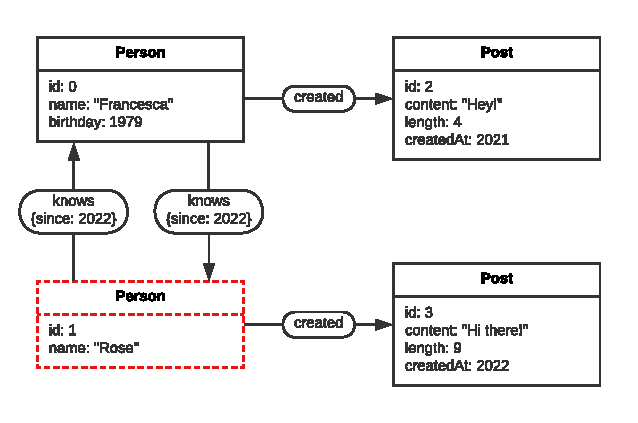
\includegraphics[width=\textwidth]{figures/conformance-basic-node.pdf}
    \caption{A \texttt{Person} is missing a \texttt{birthday}, which violates \autoref{rule:basic-node}.}
    \label{fig:conformance-basic-node}
  \end{subfigure}
  \hfill
  \begin{subfigure}[t]{0.45\textwidth}
    \centering
    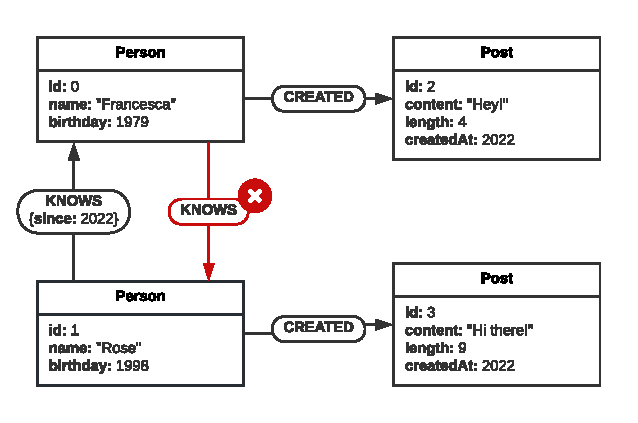
\includegraphics[width=\textwidth]{figures/conformance-basic-edge.pdf}
    \caption{A \texttt{knows} edge is missing a \texttt{since} property, which violates \autoref{rule:basic-edge}.}
    \label{fig:conformance-basic-edge}
  \end{subfigure}

  \vskip\baselineskip

  \begin{subfigure}[t]{0.45\textwidth}
    \centering
    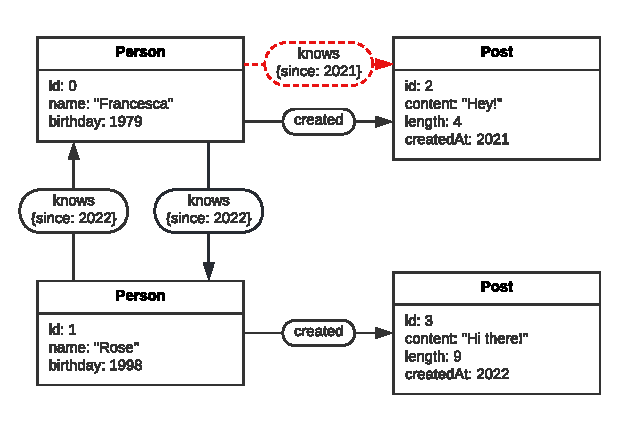
\includegraphics[width=\textwidth]{figures/conformance-basic-edge-target.pdf}
    \caption{The target of a \texttt{knows} edge is not a \texttt{Person}, which violates \autoref{rule:basic-edge}.}
    \label{fig:conformance-basic-edge-target}
  \end{subfigure}
  \hfill
  \begin{subfigure}[t]{0.45\textwidth}
    \centering
    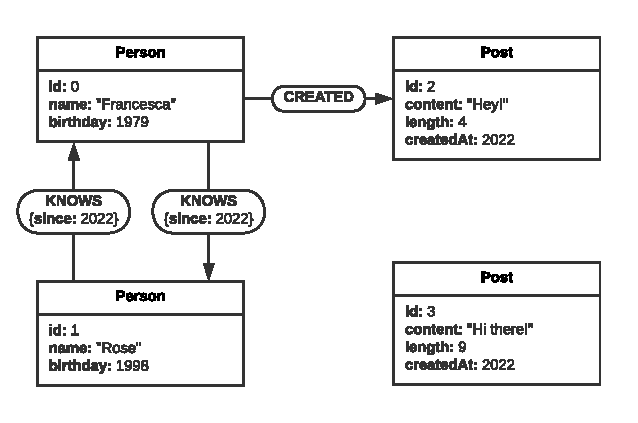
\includegraphics[width=\textwidth]{figures/conformance-basic-in.pdf}
    \caption{A \texttt{Post} is missing an incoming \texttt{created} edge, but this does not violate any rules.}
    \label{fig:conformance-basic-in}
  \end{subfigure}

  \caption{Examples of property graphs validated against the schema of \autoref{fig:pg-schema-basic}. Violating nodes and edges have a red dotted outline.}
  \label{fig:conformance-basic}
\end{figure}

\section{Cardinality constraints}
\label{sec:cardinality}

We first introduce a generalization of the existential quantifier which enables counting the number of distinct variables that satisfy a predicate.

\begin{definition}[Counting quantifier]
  The \emph{counting quantifier} is defined as follows. Given two numbers $n, m \in \N$, a predicate $P$, and a set $X$, define
  \begin{itemize}
    \item $\exists^{\geq n} x \in X : P(x) \equiv \exists x_1, \ldots, x_n \in X : P(x_1) \wedge \ldots \wedge P(x_n) \wedge \forall 1 \leq i < j \leq n : x_i \neq x_j$;
    \item $\exists^{\leq n} x \in X : P(x) \equiv \exists x_1, \ldots, x_n, x_{n+1}, \ldots, x_k \in X : P(x_1) \wedge \ldots \wedge P(x_k) \implies \forall n < i < j \leq k : x_i = x_j$;
    \item $\exists^{[n, m]} x \in X : P(x) \equiv \exists^{\geq n} x \in X : P(x) \wedge \exists^{\leq m} x' \in X : P(x')$;
    \item $\exists^{[n, *]} x \in X : P(x) \equiv \exists^{\geq n} x \in X : P(x)$.
  \end{itemize}
\end{definition}

Next, we introduce the notion of a \emph{cardinality constraint}.

\begin{definition}[Cardinality constraint]
  \label{def:cardinality-constraint}
  A \emph{cardinality constraint} is an ordered pair of intervals $([n_1, m_1], \, [n_2, m_2])$ where $n_1, n_2 \in \N$ and $m_1, m_2 \in \N^*$ with $\N = \{0, 1, 2, \ldots\}$ and $\N^* = \N \cup \{*\}$. The set of all cardinality constraints is denoted as $\mathcal{C}$.
\end{definition}

The two intervals of a cardinality constraint apply to the source and target of an edge, respectively. We also use the functions $\src$ and $\trg$ to refer to the first and second interval of a cardinality constraint, i.e. $\src([n_1, m_1], \, [n_2, m_2]) = [n_1, m_1]$ and $\trg([n_1, m_1], \, [n_2, m_2]) = [n_2, m_2]$.

Next, we revise the definitions of property graph schema and schema conformance, making use of our newly defined cardinality constraints. The following definitions subsume \autoref{def:pg-schema-basic} and~\ref{def:schema-conformance-basic}.

\begin{definition}[Property graph schema]
  \label{def:pg-schema}
  A \emph{property graph schema} is a tuple $$S = (N, E, \rho, \omega, \eta)$$ where
  \begin{itemize}
    \item $N$ is a finite set of schema nodes;
    \item $E$ is a finite set of schema edges such that $N \cap E = \emptyset$;
    \item $\rho : E \to (N \times N)$ is a total function mapping schema edges to ordered pairs of schema nodes;
    \item $\omega : (N \cup E) \to \otypes$ is a total function mapping schema objects to object types;
    \item $\eta : E \to \mathcal{C}$ is a total function mapping schema edges to cardinality constraints.
  \end{itemize}
\end{definition}

An example of a property graph schema with cardinality constraints is given in \autoref{fig:pg-schema}. Intervals such as $[n, m]$ are written as $n..m$, and $[n, n]$ is written simply as $n$, following notation established in UML~\citep{uml}. Furthermore, we use the ``look-here'' notation (as opposed to ``look-across''), meaning that the interval indicates the minimum and maximum number of edges that the node on that side of the edge must participate in. Contrary to some data modeling diagram conventions, the arrow head is unrelated to cardinality, instead it specifies the direction of an edge. Note  that every property graph that conforms to \autoref{fig:pg-schema-basic} also conforms to \autoref{fig:pg-schema}, but not the other way around.

\begin{figure}[t]
  \centering
  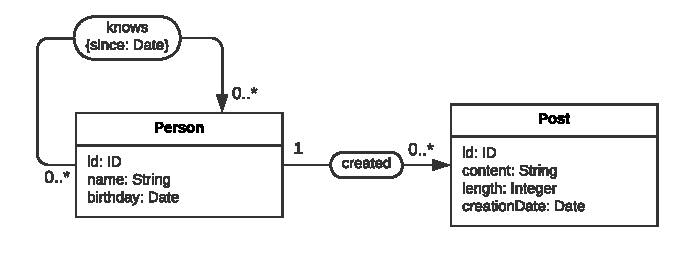
\includegraphics{figures/pg-schema.pdf}
  \caption{A property graph schema with cardinality constraints.}
  \label{fig:pg-schema}
\end{figure}

\begin{definition}[Schema conformance]
  \label{def:schema-conformance}
  Given a property graph $$G = (N, E, \rho, \lambda, \pi)$$ and a property graph schema $$S = (N', E', \rho', \omega, \eta)$$ we say that $G$ \emph{conforms} to $S$ if and only if all of the following rules hold.

  \begin{enumerate}
    \item\label{rule:node}
          Every node $n$ conforms to some schema node $n'$:
          \begin{align*}
             & \forall n \in N \; \exists n' \in N' : n \conf n'
          \end{align*}

    \item\label{rule:edge}
          Every edge $e$ conforms to some schema edge $e'$, and the source and target nodes of $e$ conform to the respective endpoints of $e'$:
          \begin{align*}
             & \forall e \in E \; \exists e' \in E' :                      \\
             & \quad e \conf e' \wedge \src(\rho(e)) \conf \src(\rho'(e'))
            \wedge \trg(\rho(e)) \conf \trg(\rho'(e'))
          \end{align*}

    \item\label{rule:out}
          If a node $n$ conforms to the source of a schema edge $e'$, it must have the right number of outgoing edges of the right type:
          \begin{align*}
             & \forall n \in N \; \forall e' \in E' :                                                        \\
             & \quad \big[n \conf \src(\rho(e')) \implies \exists^{\src(\eta(e'))} e \in E :                 \\
             & \quad\quad e \conf e' \wedge \src(\rho(e)) = n \wedge \trg(\rho(e)) \conf \trg(\rho(e'))\big]
          \end{align*}

    \item\label{rule:in}
          If a node $n$ conforms to the target of a schema edge $e'$, it must have the right number of incoming edges of the right type:
          \begin{align*}
             & \forall n \in N \; \forall e' \in E' :                                                        \\
             & \quad \big[n \conf \trg(\rho(e')) \implies \exists^{\trg(\eta(e'))} e \in E :                 \\
             & \quad\quad e \conf e' \wedge \src(\rho(e)) \conf \src(\rho(e')) \wedge \trg(\rho(e)) = n\big]
          \end{align*}
  \end{enumerate}
\end{definition}

\autoref{fig:conformance} contains some examples of property graphs which are validated against the schema of \autoref{fig:pg-schema}, taking into account the new rules.

Compared to \autoref{def:schema-conformance-basic}, \autoref{rule:node} and \ref{rule:edge} are unchanged, while \autoref{rule:out} and \ref{rule:in} enforce cardinality constraints on edges. With these new rules, we can enforce mandatory edges, i.e. a cardinality constraint of ``at least one''.

\begin{figure}[t]
  \centering
  \begin{subfigure}[t]{0.45\textwidth}
    \centering
    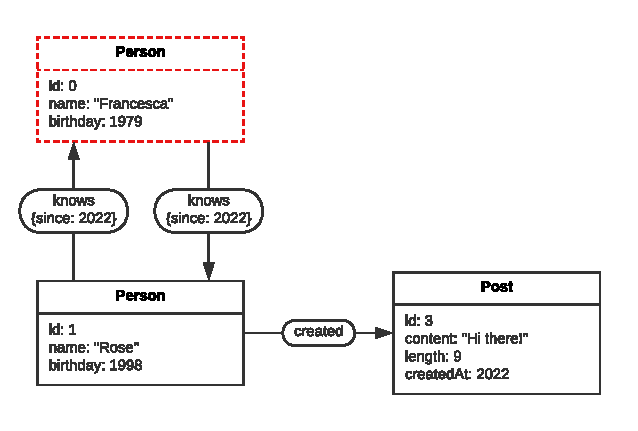
\includegraphics[width=\textwidth]{figures/conformance-out.pdf}
    \caption{Conforms to the schema. A \texttt{Person} is allowed to have created 0 \texttt{Post}s.}
    \label{fig:conformance-node}
  \end{subfigure}
  \hfill
  \begin{subfigure}[t]{0.45\textwidth}
    \centering
    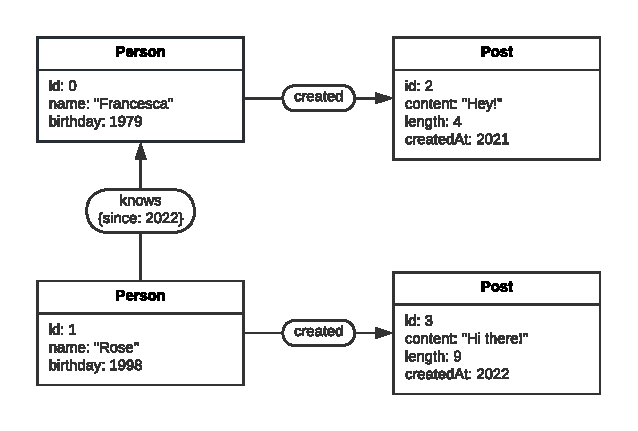
\includegraphics[width=\textwidth]{figures/conformance-out-2.pdf}
    \caption{Conforms to the schema. A \texttt{Person} is allowed to have no outgoing \texttt{knows} edges.}
    \label{fig:conformance-edge}
  \end{subfigure}

  \vskip\baselineskip

  \begin{subfigure}[t]{0.45\textwidth}
    \centering
    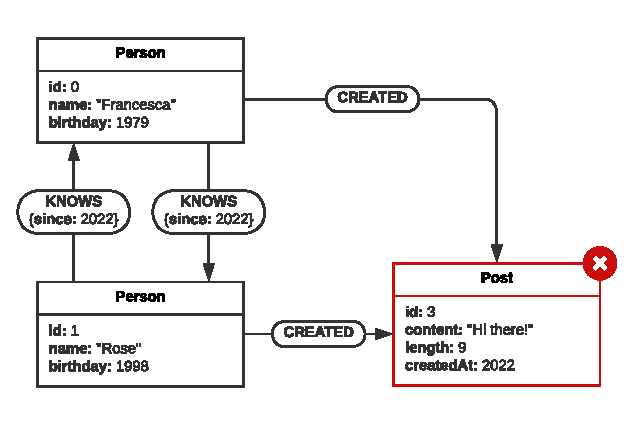
\includegraphics[width=\textwidth]{figures/conformance-too-many-in.pdf}
    \caption{This \texttt{Post} has too many incoming \texttt{created} edges, which violates \autoref{rule:in}.}
    \label{fig:conformance-edge-target}
  \end{subfigure}
  \hfill
  \begin{subfigure}[t]{0.45\textwidth}
    \centering
    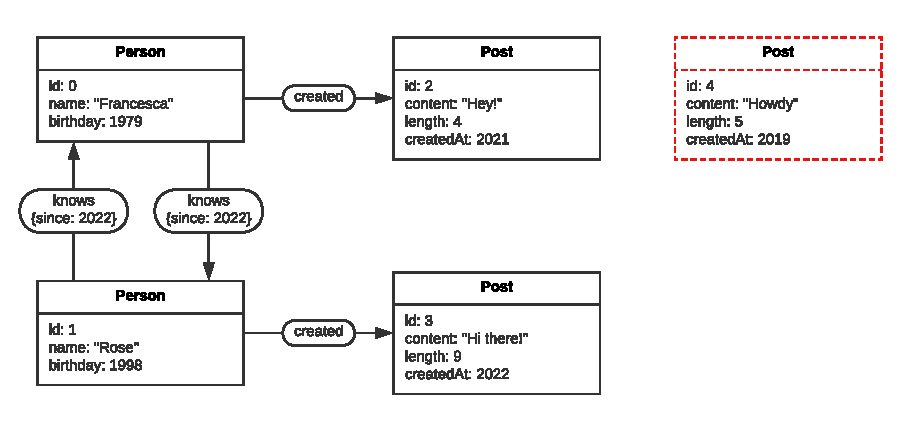
\includegraphics[width=\textwidth]{figures/conformance-in.pdf}
    \caption{A \texttt{Post} is missing an incoming \texttt{created} edge, which violates \autoref{rule:in}.}
    \label{fig:conformance-out}
  \end{subfigure}

  \caption{Examples of property graphs validated against the schema of \autoref{fig:pg-schema}. Violating nodes and edges have a red dotted outline.}
  \label{fig:conformance}
\end{figure}

\section{Optional properties}
\label{sec:optional-properties}

We revise the definition of record by adding a special property value $\undefined$, which indicates that the value of a property is not defined. The following definitions subsume Definition~\ref{def:record-basic}, \ref{def:property-conformance-basic}, \ref{def:record-type-basic}, and \ref{def:record-conformance-basic}.

\begin{definition}[Record]
  \label{def:record}
  A \emph{record} is a total function $r : \mathcal{N} \to \mathcal{V} \cup \{\undefined\}$ that maps property names to property values or the special value $\undefined$. The set of all records is denoted as $\mathcal{R}$.
\end{definition}

For a record $r$ and a property name $k \in \mathcal{N}$ such that $r(k)$ was previously undefined, we now say $r(k) = \undefined$. This can be seen as the ``default'' value of a property.

We adjust the definitions of property conformance, record type, and record conformance accordingly.

\begin{definition}[Property conformance]
  \label{def:property-conformance}
  For each property type $\ptype \in \ptypes$ there is a set $\sem{\ptype} \subseteq \mathcal{V} \cup \{\undefined\}$ that contains all property values that \emph{conform} to the type $\ptype$. We say $\ptype$ is \emph{optional} iff $\undefined \in \sem{\ptype}$. We use the notation $\ptype?$ to mark a property as optional, i.e. $\sem{\ptype?} = \sem{\ptype} \cup \{ \undefined \}$.
\end{definition}

\begin{definition}[Record type]
  \label{def:record-type}
  A \emph{record type} is a total function $\rtype : \mathcal{N} \to \ptypes$ that maps property names to a property type.
  % We denote such record types as $\langle a_1 : \rtype_1, \ldots, a_n : \rtype_n \rangle$.
\end{definition}

\begin{definition}[Record conformance]
  \label{def:record-conformance}
  We say that a record $r$ \emph{conforms} to a record type $\rtype$, denoted $r \in \sem{\rtype}$, if and only if for each property name $k \in \mathcal{N}$ it holds that $r(k) \in \sem{\rtype(k)}$.
\end{definition}

\section{Open record types}

It may be desirable to allow a record to have properties with any name or any value. Such \emph{open record types} can already be expressed under the current definitions. For a record type $\rtype$, we can allow properties with any name by setting $\rtype(k) = \ptype?$ for all (previously unspecified) property names $k \in \mathcal{N}$, where $\ptype$ is an arbitrary property type. Note that there may be infinitely many such $k$, so in practice we may want to have a special syntax to express this. We can allow these properties to have any value by choosing a $\ptype$ such that $\sem{\ptype} = \mathcal{V}$, or we can restrict them to a subset of $\mathcal{V}$.

\section{Discussion}

% TODO: lack of key constraints?
% TODO: suggest richer constraint language
% TODO: can we allow edge to any other node?
% TODO: multigraph can cause unexpected results, e.g. node can conform to minimum cardinality by having multiple edges to the same node (is this desirable? in some situations it might be, e.g. chemistry)
% TODO: multiple schema nodes with same label: could model mutually exclusive properties?

Our schema formalisms come with a number of limitations. First, it is not possible to specify constraints over a graph pattern larger than two neighboring nodes and the edge between them. For example, say we want to allow a person to drive a car, but only when they have a driver's license. \autoref{fig:drivers-license} depicts a schema that models these entities and their relations this using three nodes and two edges. Unfortunately, it is not possible to prevent a person from driving a car without having a driver's license. This illustrates the limited scope of the constraints that we can specify.

\begin{figure}[t]
  \centering
  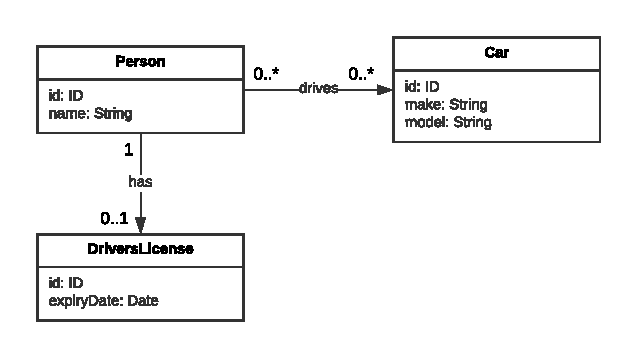
\includegraphics{figures/drivers-license.pdf}
  \caption{A schema consisting of three nodes and two edges. While we can specify constraints on edge cardinalities, we cannot ensure that a person only drives a car if they have a driver's license.}
  \label{fig:drivers-license}
\end{figure}

% Alternatively, we can have two \texttt{Person} nodes, where one requires having a \texttt{DriversLicense} and allows owning 0 or more \texttt{Car}s, and the other does not allow owning a \texttt{Car}. This would indeed prevent a situation where a \texttt{Person} owns a \texttt{Car}, but does not have a \texttt{DriversLicense}. However, ...

% However, this breaks down when we add constraints that depend on the uniqueness of a \texttt{Person}. For example, say we want to model that a Person has exactly one Passport, and every Passport is associated with exactly one Person.
% FIXME: actually, this seems possible, as long as everything is the same for both Person nodes

% Node with any label: create a node for every combination of labels (but then we can't express there should be an edge to "at least one" of them). Solution: union types? Look into type theory again

% Furthermore, it is not possible to have a single object type that allows two different label sets. Hence, it is not possible to have optional labels, i.e. the object type $\otype = (\{\texttt{Vehicle}, \texttt{Car}\}, \langle \texttt{make} : \texttt{string} \rangle)$ requires that the labels \texttt{Vehicle} and \texttt{Car} are both present, just having \texttt{Car} is not enough. Of course, it is possible to have two schema objects like $\otype_1 = (\{\texttt{Car}\}, \langle \texttt{make} : \texttt{string} \rangle)$ and $\otype_2 = (\{\texttt{Vehicle}, \texttt{Car}\}, \langle \texttt{make} : \texttt{string} \rangle)$. However, then it is not possible to specify that every \texttt{Employee} must have exactly one outgoing \texttt{OWNS} edge to a node conforming to either $\otype_1$ or $\otype_2$.

% TODO: In general, it's not possible to say that an object must conform to type 1 OR type 2 (union type). Problem with labels follows from that. But also union of two records is not possible.

% TODO: It's also not possible to say that there may only exist one edge between the same two nodes, or to enforce that a node has two edges to different nodes (mutual exclusion?)

Furthermore, subtype relations cannot be expressed in general. To see the problem, consider the schema depicted in \autoref{fig:subtyping}. How could we express this using our schema formalism? An attempt is given in \autoref{fig:subtyping-ours}, where properties of the supertype \texttt{Message} are copied and distributed over all its subtypes, and the edge from \texttt{Comment} to \texttt{Message} is accompanied by an edge from \texttt{Comment} to Post and from \texttt{Comment} to itself. While the properties are modeled correctly in this case, it breaks down when we look at the cardinalities.

In \autoref{fig:subtyping}, a constraint is specified which we can express in words as ``every \texttt{Comment} is a reply of exactly one \texttt{Message} (or a subtype of \texttt{Message})''. However, it is not possible to specifiy such a constraint without subtype relations, as illustrated by \autoref{fig:subtyping-ours}. This solution allows \texttt{Comment}s which are not a reply to anything, or which are a reply to more than one thing. Then again, if we disregard the cardinality constraints, the two schemas are equivalent. This example shows that our schema formalism can be used to model some but not all subtype relations.

\begin{figure}[t]
  \centering
  \begin{subfigure}[t]{0.45\textwidth}
    \centering
    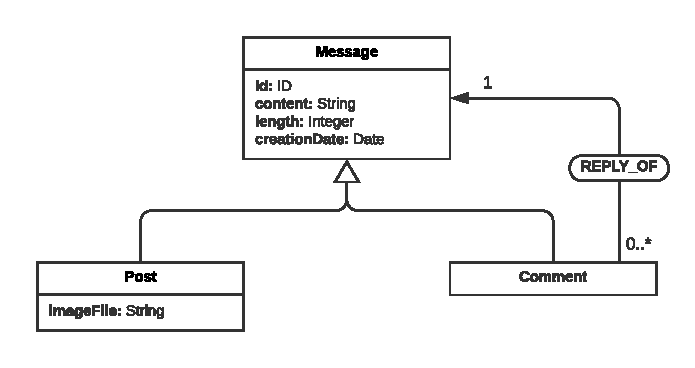
\includegraphics[width=\textwidth]{figures/subtyping.pdf}
    \caption{A schema with a subtype relation. The arrow with solid white head indicates a ``subtype of'' relation.}
    \label{fig:subtyping}
  \end{subfigure}
  \hfill
  \begin{subfigure}[t]{0.45\textwidth}
    \centering
    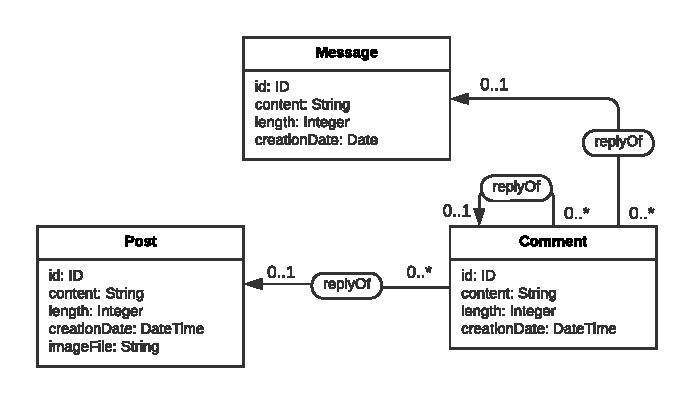
\includegraphics[width=\textwidth]{figures/subtyping-ours.pdf}
    \caption{An attempt to express the same schema without subtype relations. Note that this schema is strictly more permissive than~(a).}
    \label{fig:subtyping-ours}
  \end{subfigure}
  \caption{A schema consisting of a supertype with two subtypes which cannot be modeled using our schema formalism. Any property graph that conforms to~(a) also conforms to~(b), but not the other way around.}
\end{figure}

\chapter{Experimental Study}
\label{sec:experiment}

We have defined a property graph schema formalism which is capable of expressing constraints in commonly used conceptual data modeling methods. Next, we analyze the practical feasibility of our approach. We aim to answer the question: what is the cost of determining property graph schema conformance using currently available graph database systems? First, we investigate the schema capabilities of three existing graph database sytems. Second, we describe how these systems can be extended to support all kinds of constraints that can be specified in our schema formalism. Third, we analyze the performance of our prototypical implementation in several realistic scenarios.

\section{State of the art}
\label{sec:sota}

Current property graph database systems vary in their support and philosophy around schema. Most embrace the flexibility of the property graph data model by supporting optional, partial, or implicit schemas. Others require the schema to be fully specified in advance. We take a closer look at three of the most popular property graph databases: Neo4j, JanusGraph, and TigerGraph.

A summary of the differences in schema capabilities is shown in \autoref{tab:schema-comparison}. We elaborate here on the meaning of the listed schema features. Mandatory property constraints express that some property must exist on an object. Allowed property constraints express that no properties may exist, other than the ones explicitly specified. Endpoint constraints express that edges may not connect nodes which do not conform to some specified types. Data type constraints express that the value of a property must be of a particular data type. Maximum and mimumum cardinality constraints express that a node must have some number of incoming or outgoing edges of a particular type. Property uniqueness constraints express that no two nodes may have the same value for a particular property (note that a property is a key if it is mandatory and unique).

Referring back to our definition of schema conformance (\autoref{def:schema-conformance}), we can see how each of the constraints in \autoref{tab:schema-comparison} can be linked to a conformance rule. Mandatory and allowed properties are captured by our notion of record conformance (\autoref{def:record-conformance}), which corresponds to \autoref{rule:node}. Endpoint constraints correspond to \autoref{rule:edge}. Data type constraints are captured by our notion of object conformance (\autoref{def:object-conformance}), and correspond to \autoref{rule:node}. Cardinality constraints correspond to \autoref{rule:out} and \ref{rule:in}.

\begin{table}[t]
  \centering
  \begin{tabularx}{\textwidth}{|X|l|l|l|l|l|}
    \hline
                & \textbf{Neo4j}     & \textbf{Neo4j}      & \textbf{TigerGraph} & \textbf{JanusGraph} & \textbf{Ours} \\
                & \textbf{Community} & \textbf{Enterprise} &                     &                     &               \\
    \hline
    Mandatory   & \no                & \yes                & \no                 & \yes                & \yes          \\
    properties  &                    &                     &                     &                     &               \\
    \hline
    Allowed     & \no                & \no                 & \yes                & \no                 & \yes          \\
    properties  &                    &                     &                     &                     &               \\
    \hline
    Endpoint    & \no                & \no                 & \yes                & \yes                & \yes          \\
    constraints &                    &                     &                     &                     &               \\
    \hline
    Data type   & \no                & \no                 & \yes                & \yes                & \yes          \\
    constraints &                    &                     &                     &                     &               \\
    \hline
    Maximum     & \no                & \no                 & \yes*               & \no                 & \yes          \\
    cardinality &                    &                     &                     &                     &               \\
    \hline
    Minimum     & \no                & \no                 & \no                 & \no                 & \yes          \\
    cardinality &                    &                     &                     &                     &               \\
    \hline
    Property    & \yes               & \yes                & \no                 & \yes                & \no           \\
    uniqueness  &                    &                     &                     &                     &               \\
    % \hline
    % Subtyping   & \no & \no & \no & \no & \no \\
    \hline
  \end{tabularx}
  \caption{Comparison of schema capabilities of property graph database systems and our schema formalism. *: only one-to-one, one-to-many, etc.}
  \label{tab:schema-comparison}
\end{table}

Next, we detail the differences between the three database systems in our scope with respect to their data models and schema capabilities.

% TODO: mention query languages

\paragraph{Neo4j.} Being one of the first to adopt the property graph data model, Neo4j has grown to become the most popular graph database engine today\footnote{\url{https://db-engines.com/en/ranking/graph+dbms} (accessed July 2022)}. Their data model differs from ours in that edges can only have a single label, while nodes can have multiple.

Neo4j's approach to schema is primarily implicit: after inserting data, the user can construct a schema that describes the data using built-in functions. In addition, some constraints can be explicitly specified, namely existence of mandatory properties (enterprise edition only), uniqueness of property values, and key constraints.

\paragraph{JanusGraph.} Originating from the open source Titan project, JanusGraph is a continuation of the effort to create a distributed and highly scalable graph database. In their data model, nodes and edges always have one label. Properties can have sets and lists as values, and there may exist multiple properties with the same key on the same node. Furthermore, properties themselves can have properties. In this sense, the data model is like a blend of property graphs and RDF \citep{pan2009rdf}.

JanusGraph has the largest set of schema features among all systems we came across. Similarly to Neo4j, JanusGraph can automatically generate a schema during operation. However, this functionality can be disabled, in which case the schema must be explicitly defined. There is built-in support for specifying which node labels, edge labels, and property names may exist. Furthermore, it can be specified which properties may exist depending on the label of a node or edge. Property values are restricted to a data type and may be single-valued or multi-valued (lists or sets). In addition, the types of the source and target nodes that may be connected by an edge with a particular label can be constrained. Edge cardinality can be constrained to one-to-one, one-to-many, many-to-one, many-to-many, or ``simple'' (at most one edge of a particular label between any pair of nodes). Finally, there are features to support static (immutable) nodes, time-to-live (TTL), and unidrectional edges which can only be traversed from source to target.

All of JanusGraph's schema features are centered around specifying what is allowed in the graph, but mandatory properties and edges are not supported. Cardinality constraints are supported, but not to the full extent of our definition. To be precise, JanusGraph can impose constraints on the maximum edge cardinality, but not the minimum. For example, a many-to-one schema edge ensures that every target node has at most one incoming edge of a particular type, but does not prevent a target node from having no incoming edges.

\paragraph{TigerGraph.} A unique aspect of TigerGraph \citep{deutsch2019tigergraph} is that it is schema-first: the entire schema must be specified before a database is instantiated. This allows for more powerful optimizations, building on decades of research on relational databases. In TigerGraph's data model, nodes and edges have exactly one label, but nodes can be associated with any number of \emph{tags}, which are conceptually similar to labels. Edges can be directed or undirected.

TigerGraph's schema is strict, in the sense that every node label, edge label, and property must be explicitly defined. All properties are mandatory and have a fixed data type, which may be singular or multi-valued. There are no null values; if a property value is missing during insertion, a default value is set. All nodes have a primary key, which may be a single property or a composite key. Schema edges must specify a source and target node type, though it is possible to specify multiple types on either side. By default, directed edges can only be traversed from source to target, though a reverse edge can be automatically constructed if desired.

\section{Workloads}
\label{sec:workloads}

\paragraph{Objective.} We consider two variants of the schema validation problem:

\begin{itemize}
  \item \textbf{Boolean validation:} given a graph and a schema, determine whether the graph conforms to the schema or not.
  \item \textbf{Full validation:} given a graph and a schema, find all graph objects which cause a violation of at least one of the rules of schema conformance.
\end{itemize}

While a Boolean validation method may be sufficient in some situations, full validation is required when we want to explain why a graph does not conform. Boolean validation is a strictly easier problem because we can stop as soon as we find a single violation, while full validation always requires at least one full scan of the graph.

\paragraph{Datasets.} Our schema validation methods are applied to two datasets:

\begin{itemize}
  \item The \textbf{Recommendations Graph}\footnote{\url{https://github.com/neo4j-graph-examples/recommendations}} is a relatively small dataset with a simple schema, provided by Neo4j. It contains movies, actors, directors, and users who rate movies. The schema is given in \autoref{fig:schema-recommendations}. This dataset is intended as a working example for people who want to explore the functionality of a graph database. The small size makes it suitable as a proof-of-concept for our schema validation methods.
  \item The \textbf{LDBC Social Network Benchmark} (SNB) \citep{angles2020snb} was designed to evaluate graph-like data management technologies in a realistic setting. The dataset consists of users, messages, likes, and other concepts that can be found in the domain of social networks. The schema is of moderate size, and is given in \autoref{fig:schema-snb}. The data is made available at various scales, ranging from less than a gigabyte to a terrabyte of raw data. We run multiple tests with scale factor 0.1, 0.3, and 1. This lets us study how our solution scales with the size of the data.
\end{itemize}

A comparison of the datasets is given in \autoref{tab:dataset-comparison}.

% TODO: SF0.3 and 1 statistics
\begin{table}[t]
  \centering
  \begin{tabular}{|l|r|r|r|r|r|}
    \hline
    \textbf{Dataset} & $\bf{|N|}$ & $\bf{|E|}$ & $\bf{|N'|}$ & $\bf{|E'|}$ & \textbf{Raw} \\
    \hline
    Recommenations   & 28,863     & 166,261    & 6           & 6           & 22 MB        \\
    \hline
    SNB (SF0.1)      & 327,588    & 1,477,965  & 14          & 20          & 100 MB       \\
    % \hline
    % SNB (SF0.3) & 0 & 0 & 0 & 0 & 0\\
    % \hline
    % SNB (SF1)  & 0 & 0 & 0 & 0 & 0\\
    \hline
  \end{tabular}
  \caption{A comparison of the datasets used in the experiment. $|N|$ and $|E|$ represent the number of nodes and edges. $|N'|$ and $|E'|$ represent the number of schema nodes and schema edges. The raw size is measured as the combined size of all CSV files.}
  \label{tab:dataset-comparison}
\end{table}

\begin{figure}[t]
  \centering
  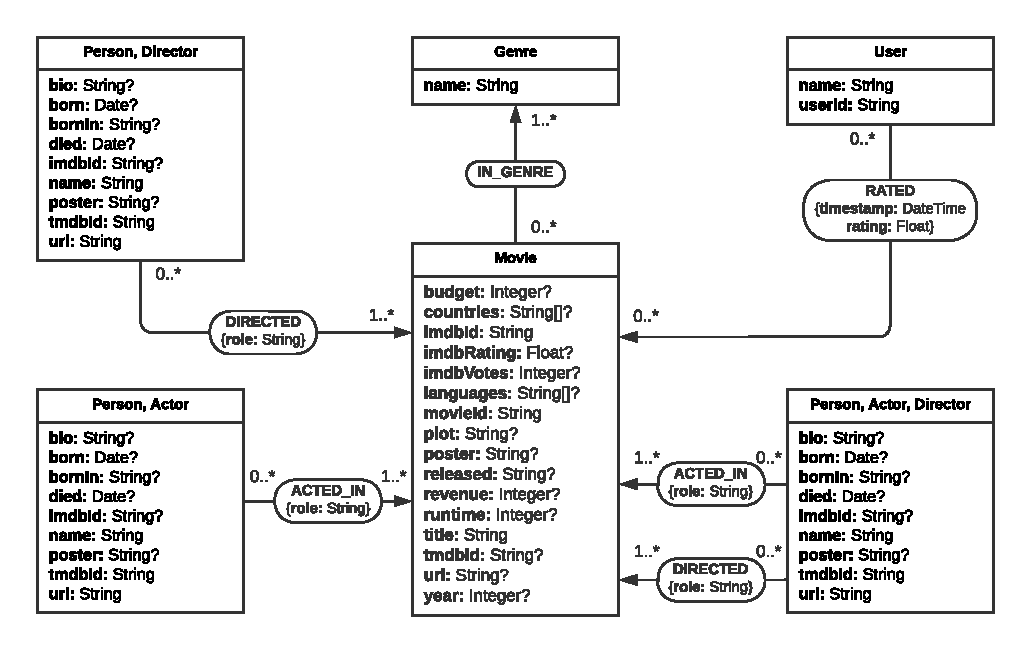
\includegraphics[width=\textwidth]{figures/schema-recommendations.pdf}
  \caption{Schema of the Recommendations Graph dataset. This schema was constructed manually by analyzing the data.}
  \label{fig:schema-recommendations}
\end{figure}

\begin{figure}[t]
  \centering
  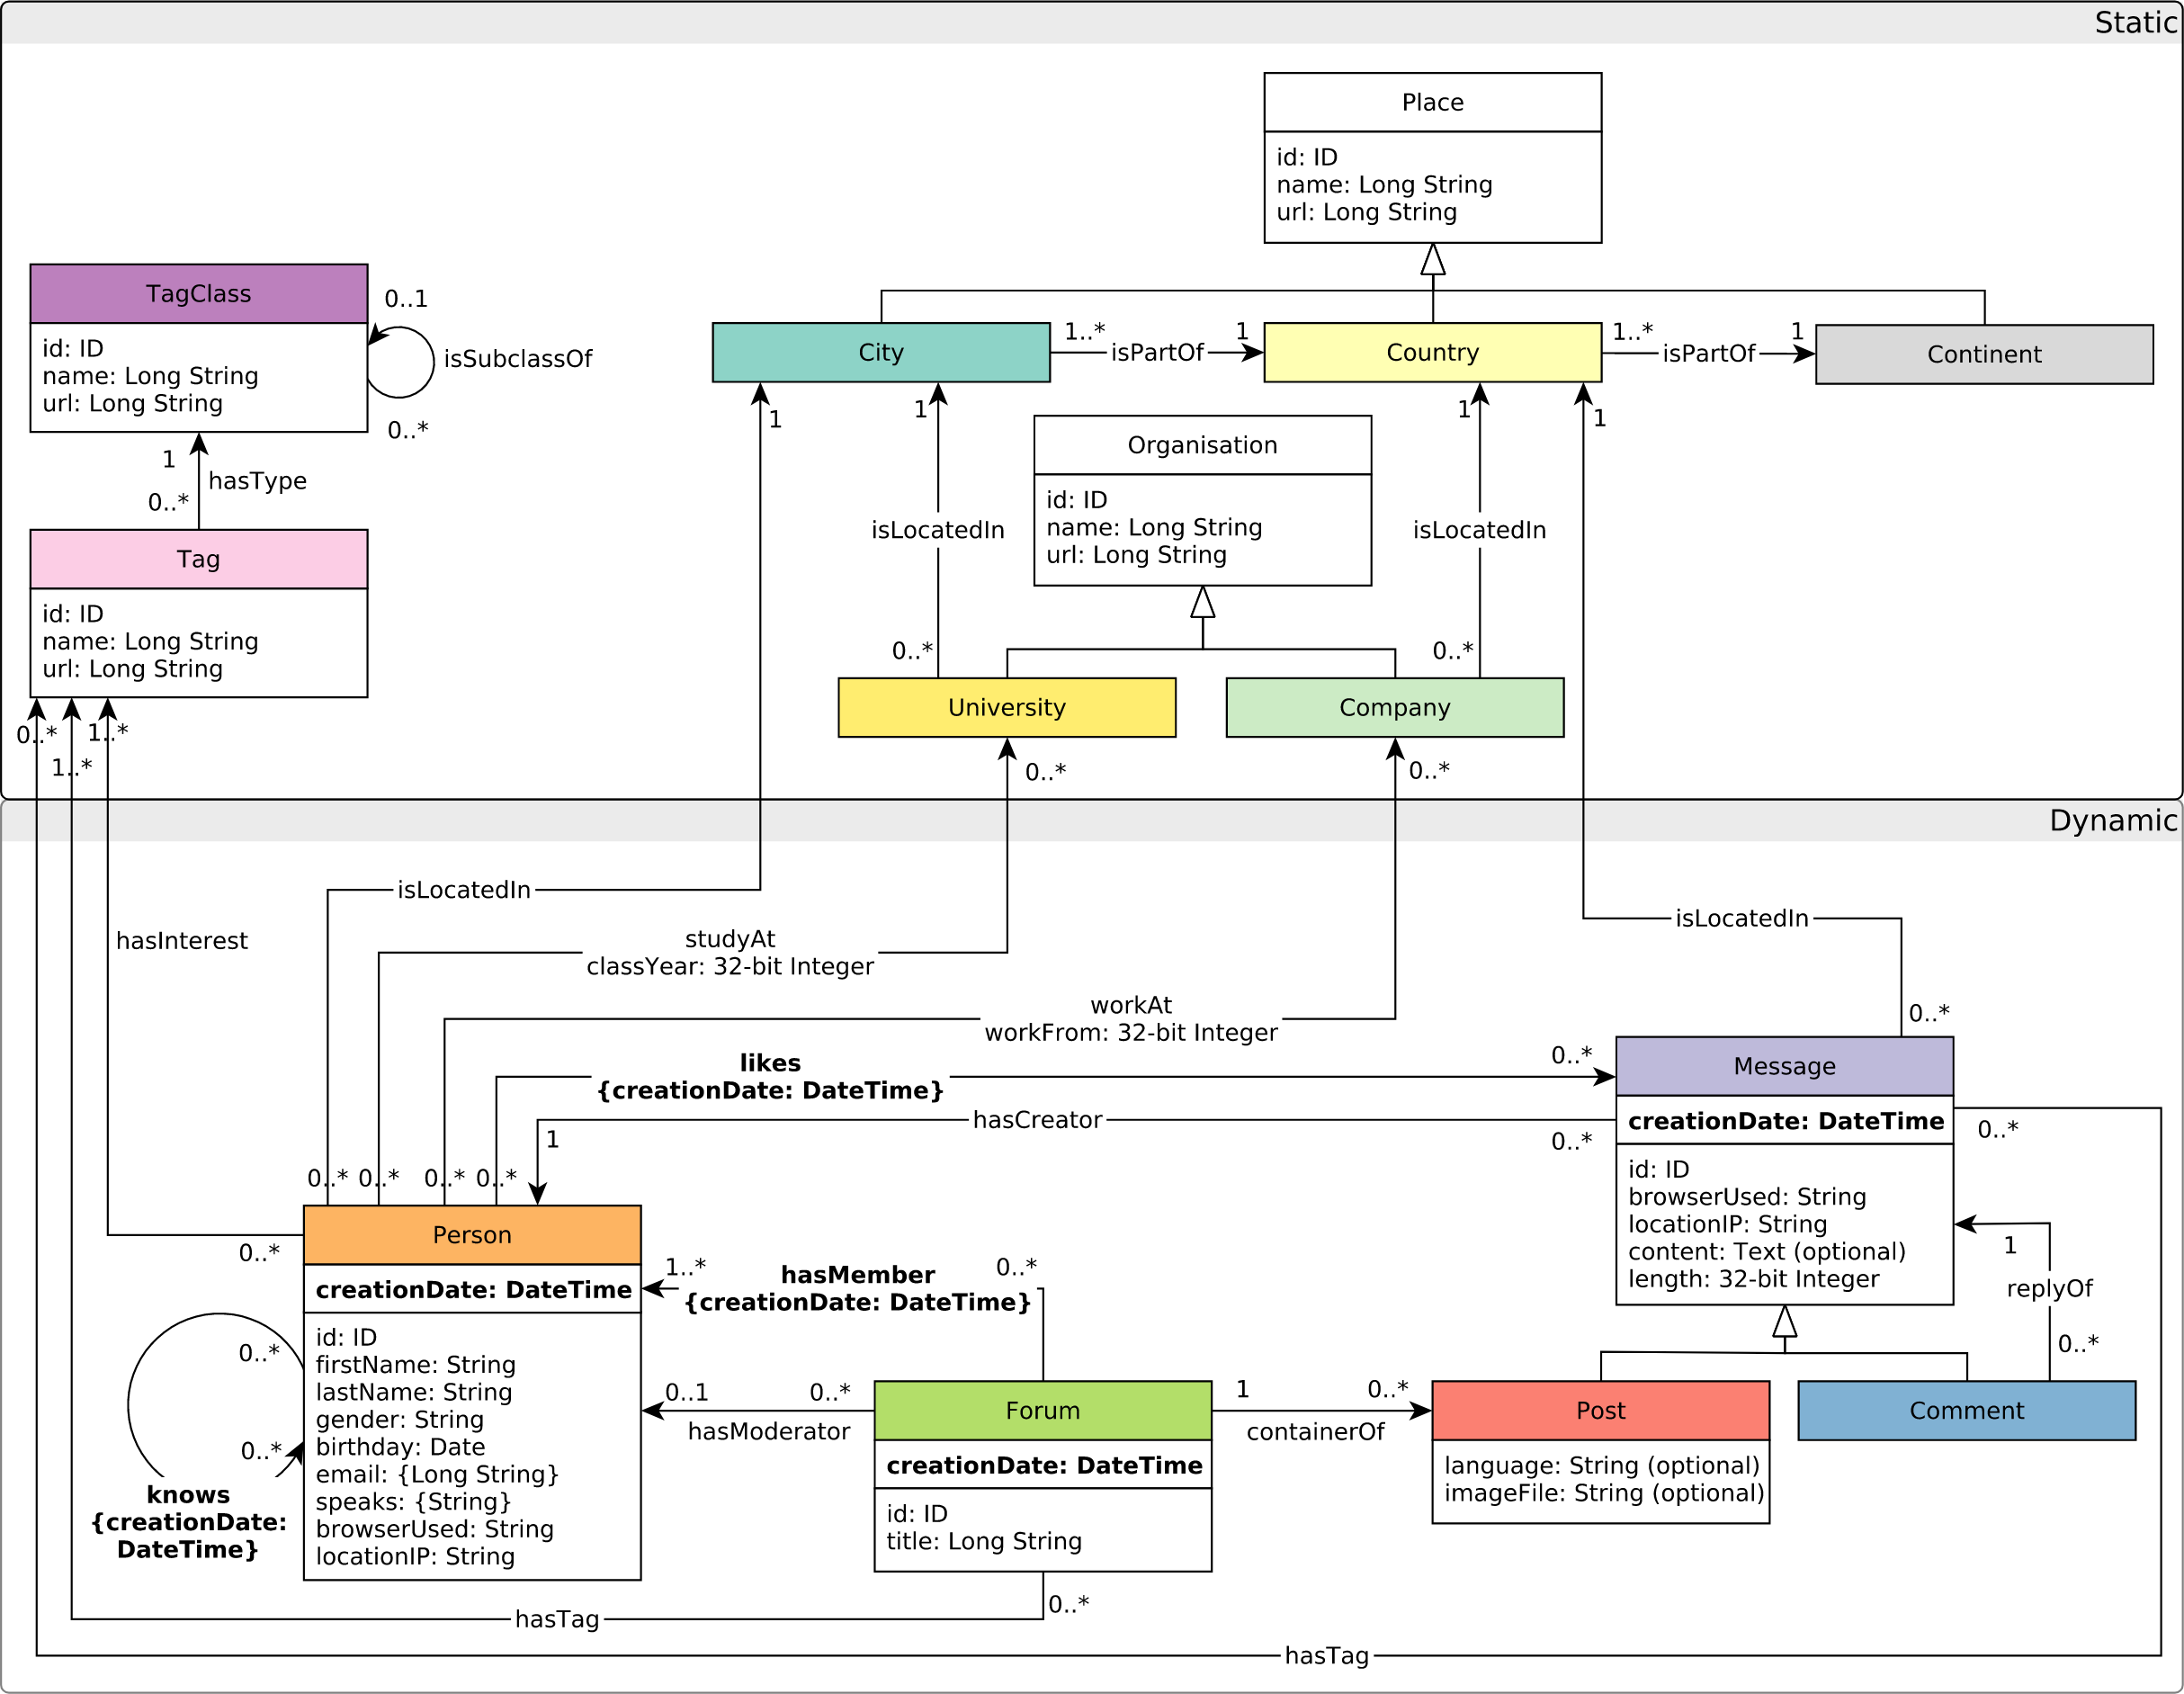
\includegraphics[width=\textwidth]{figures/schema-snb.png}
  \caption{Schema of the SNB dataset (source: \citet{angles2020snb}).}
  \label{fig:schema-snb}
\end{figure}

\paragraph{Assumptions.} To reduce the complexity of the implementation, we assume that the set of labels of a schema object functionally determines the record type of that schema object. Recall that every object must conform to a schema object (\autoref{rule:node} and \ref{rule:edge}). This implies that if an object has the same set of labels as a schema object, it must conform to that schema object (since there exists no schema object with the same label set and a different record type). We find that this assumption holds in many domains, including the datasets we study.

Under this assumption, we can simplify the rules of conformance. Informally:

\begin{enumerate}
  \item
  \begin{enumerate}
    \item\label{rule:simp-node-labels}
    Every node has the same set of labels as some schema node.
    \item\label{rule:simp-node-mandatory-props}
    All mandatory properties exist on the node.
    \item\label{rule:simp-node-allowed-props}
    The node has no properties that are not allowed.
    \item\label{rule:simp-node-datatype}
    All node properties have a value of the right type.
  \end{enumerate}
  \item
  \begin{enumerate}
    \item\label{rule:simp-edge-labels}
    Every edge has the same set of labels as some schema edge.
    \item\label{rule:simp-edge-mandatory-props}
    All mandatory properties exist on the edge.
    \item\label{rule:simp-edge-allowed-props}
    The edge has no properties that are not allowed.
    \item\label{rule:simp-edge-datatype}
    All edge properties have a value of the right type.
    \item\label{rule:simp-edge-endpoints}
    Both endpoints of the edge have the right labels.
  \end{enumerate}
  \item\label{rule:simp-card-out}
  Every node has the right number of outgoing edges with the right labels.
  \item\label{rule:simp-card-in}
  Every node has the right number of incoming edges with the right labels.
\end{enumerate}

\section{Implementation}

Having investigated existing property graph database systems, we find that none are currently able to enforce all kinds of constraints that can be expressed with our schema formalism, in particular cardinality constraints. In this section, we describe how these systems can be extended to support all schema features. Where possible, we make use of the schema functionality exposed by the database engine. For conformance rules that cannot be checked this way, we provide queries.

% TODO: why queries instead of in-engine implementation?

% TODO: examples

\paragraph{Neo4j.} We start by using the built-in schema functionality that Neo4j offers. To ensure the existence of mandatory properties (\autoref{rule:simp-node-mandatory-props} and \ref{rule:simp-edge-mandatory-props}), we use Neo4j's \texttt{CONSTRAINT} functionality, which lets us specify which properties are mandatory for nodes and edges with a particular label set (Enterprise edition only). An example is given in \autoref{lst:neo4j-mandatory-props}.

\begin{figure}[H]
\begin{lstlisting}[
  language=Cypher,
  caption={Creation of constraints which require the existence of some mandatory properties on \texttt{Movie} nodes.},
  label=lst:neo4j-mandatory-props
]
CREATE CONSTRAINT FOR (m:Movie) REQUIRE m.imdbId IS NOT NULL;
CREATE CONSTRAINT FOR (m:Movie) REQUIRE m.movieId IS NOT NULL;
CREATE CONSTRAINT FOR (m:Movie) REQUIRE m.title IS NOT NULL;
\end{lstlisting}
\end{figure}

Next, we tackle the validation of the node and edge labels (\autoref{rule:simp-node-labels} and \ref{rule:simp-edge-labels}) using Cypher queries. Neo4j provides functions \texttt{db.labels()} and \texttt{db.relationshipTypes()}, which respectively return a list of all node and edge labels that exist in the database. Unfortunately, these functions do not tell us which \emph{combinations} of labels exist. Since nodes can have multiple labels, we must fall back to a \texttt{MATCH} query which checks that every node has one of the allowed combinations of labels (see \autoref{lst:neo4j-node-labels}). Since edges in Neo4j can only have one label (called a \emph{relationship type}), we can use \texttt{db.relationshipTypes()} to determine if there exist any edges with a label that is not allowed (see \autoref{lst:neo4j-edge-labels}). This is sufficient for Boolean validation, but if we want to find out precisely which edges have an illegal label, we again need to use a \texttt{MATCH} query.

\begin{figure}[H]
\begin{lstlisting}[
  language=Cypher,
  caption={A query to find all nodes that have a label set that is not allowed.},
  label=lst:neo4j-node-labels
]
WITH [["Actor", "Person"], ["Movie"], ["User"], ...] AS allowedNodeLabelSets
MATCH (n)
WHERE NOT labels(n) IN allowedNodeLabelSets
RETURN n
\end{lstlisting}
\end{figure}

\begin{figure}[H]
\begin{lstlisting}[
  language=Cypher,
  caption={A query to check if there are any edge labels that are not allowed. Note that this query returns a Boolean, and does not explain which edges have an illegal label.},
  label=lst:neo4j-edge-labels
]
WITH ["ACTED_IN", "DIRECTED", ...] AS allowedEdgeLabels
CALL db.relationshipTypes() YIELD relationshipType AS allTypes
RETURN all(type IN collect(allTypes) WHERE type IN allowedEdgeLabels)
\end{lstlisting}
\end{figure}

Next, we look at the properties. The functions \texttt{db.schema.nodeTypeProperties()} and \texttt{db.schema.relTypeProperties()} provide useful information about the properties that exist on nodes and edges, as well as their data types. This allows us to determine if there are any nodes or edges that have properties that are not allowed (\autoref{rule:simp-node-allowed-props} and \ref{rule:simp-edge-allowed-props}), or have the wrong data type (\autoref{rule:simp-node-datatype} and \ref{rule:simp-edge-datatype}). See \autoref{lst:neo4j-allowed-props-boolean} for an example of such a query. Again, if we want to find the violating objects, we need to use a \texttt{MATCH} query that scans all properties of all objects in the database. In that case, we use the \texttt{apoc.meta.type()} function (provided by the APOC library\footnote{\url{https://neo4j.com/labs/apoc/}}) to get the data type of a property at query-time. \autoref{lst:neo4j-allowed-props-full} shows an example.

\begin{figure}[H]
\begin{lstlisting}[
  language=Cypher,
  caption={A query to check if there are any \texttt{User} nodes with properties that are not allowed or have the wrong datatype. If the result is empty, there are no violations.},
  label=lst:neo4j-allowed-props-boolean
]
CALL db.schema.nodeTypeProperties() YIELD nodeLabels, propertyName, propertyTypes
WHERE "User" IN nodeLabels AND (
    NOT propertyName IN ["userId", "name"]
    OR propertyName = "userId" AND propertyTypes <> ["String"]
    OR propertyName = "name" AND propertyTypes <> ["String"]
)
RETURN nodeLabels, propertyName, propertyTypes
\end{lstlisting}
\end{figure}

\begin{figure}[H]
\begin{lstlisting}[
  language=Cypher,
  caption={A query to find all \texttt{User} nodes with properties that are not allowed or have the wrong datatype.},
  label=lst:neo4j-allowed-props-full
]
WITH {
    userId: "STRING",
    name: "STRING"
} AS propertyTypes
MATCH (n:User)
WHERE NOT all(pKey IN keys(n) WHERE pKey IN keys(propertTypes) AND apoc.meta.type(n[pKey]) = propertyTypes[pKey])
RETURN n
\end{lstlisting}
\end{figure}

To check \autoref{rule:simp-edge-endpoints}, we do a \texttt{MATCH} query for every edge label, and look at the source and target nodes. For every edge, there must exist a schema edge such that the labels of the source and target in the data match the labels of the source and target in the schema.
% An example of such a query is shown in \autoref{lst:neo4j-endpoints}.

\begin{figure}[H]
\begin{lstlisting}[
  language=Cypher,
  caption={A query that finds all \texttt{ACTED\_IN} edges where the endpoints have the wrong label. Note that the source node \texttt{n} may have additional labels.},
  label=lst:neo4j-endpoints
]
MATCH (n)-[e:ACTED_IN]->(m)
WHERE NOT "Actor" IN labels(n) OR NOT labels(m) = ["Movie"]
RETURN e;
\end{lstlisting}
\end{figure}

Finally, we check the cardinality constraints (\autoref{rule:simp-card-out} and \ref{rule:simp-card-in}). Since the schemas of our datasets only contain ``one or more'' constraints, a simple \texttt{MATCH} query for each relevant node label is sufficient. See \autoref{lst:neo4j-mandatory-edges} for an example.
% If the cardinality constraint is more specific (say, exactly 3), then we can use the \texttt{size()} function to count the number of matches of the pattern.

\begin{figure}[H]
\begin{lstlisting}[
  language=Cypher,
  caption={A query to find \texttt{ACTOR} nodes that are missing a mandatory \texttt{ACTED\_IN} edge.},
  label=lst:neo4j-mandatory-edges
]
MATCH (a:Actor)
WHERE NOT (a)-[:ACTED_IN]->(:Movie)
RETURN a;
\end{lstlisting}
\end{figure}

\paragraph{JanusGraph.} The additional schema features that JanusGraph provides allow us to enforce most conformance rules at the time of schema definition, preventing any non-conforming data from being inserted. The complete set of allowed node and edge labels (\autoref{rule:simp-node-labels} and \ref{rule:simp-edge-labels}) are defined using \texttt{makeVertexLabel()} and \texttt{makeEdgeLabel()}. If a schema object has more than one label, we concatenate them to form a single label. This does not affect the semantics (as long as the order of concatenation is consistent), since we only ever check for equality of label sets.

For each edge label, the method \texttt{addConnection()} lets us specify the allowed labels of the edge endpoints (\autoref{rule:simp-edge-endpoints}). The maximum cardinality for an edge label is can be set with \texttt{multiplicity()}, but this does not provide any guarantees on minimum cardinality.

The complete set of allowed property names is defined using \texttt{makePropertyKey()}. Next, each label is mapped to a set of property names using \texttt{addProperties()}. This prevents objects from having properties that are not allowed (\autoref{rule:simp-node-allowed-props} and \ref{rule:simp-edge-allowed-props}). The data type of each property is defined using \texttt{dataType()} (\autoref{rule:simp-node-datatype} and \ref{rule:simp-edge-datatype}). In JanusGraph, there cannot exist two properties with the same name and different data type. If this is desired, the property name must be disambiguated, which could be achieved by prefixing it with the object label.

For an example of all of JanusGraph's built-in schema functions working together, have a look at \autoref{lst:janusgraph-schema}.

\begin{figure}[H]
\begin{lstlisting}[
  language=Java,
  caption={A fragment of the Recommendations schema, expressed using JanusGraph's schema methods. Mandatory properties and cardinality constraints cannot be validated this way. The \texttt{Multiplicity.SIMPLE} configuration ensures there is no more than one \texttt{ACTED\_IN} edge between any given actor and movie.},
  label=lst:janusgraph-schema
]
// Vertex labels
VertexLabel Actor = mgmt.makeVertexLabel("Actor").make();
VertexLabel Movie = mgmt.makeVertexLabel("Movie").make();
// Edge labels
EdgeLabel ACTED_IN = mgmt.makeEdgeLabel("ACTED_IN").multiplicity(Multiplicity.SIMPLE).make();
// Edge connections
mgmt.addConnection(ACTED_IN, Actor, Movie);
// Property keys
PropertyKey nameKey = mgmt.makePropertyKey("name").dataType(String.class).make();
PropertyKey titleKey = mgmt.makePropertyKey("title").dataType(String.class).make();
PropertyKey revenueKey = mgmt.makePropertyKey("revenue").dataType(Long.class).make();
PropertyKey roleKey = mgmt.makePropertyKey("role").dataType(String.class).make();
// Property mapping
mgmt.addProperties(Actor, nameKey);
mgmt.addProperties(Movie, titleKey, revenueKey);
mgmt.addProperties(ACTED_IN, roleKey);
\end{lstlisting}
\end{figure}

The remaining rules cannot be fully enforced by JanusGraph's schema, so we write queries to achieve this. Missing mandatory properties (\autoref{rule:simp-node-mandatory-props} and \ref{rule:simp-edge-mandatory-props}) are found using a combination of \texttt{hasLabel} and \texttt{hasNot} steps of the Gremlin query language (see \autoref{lst:janusgraph-mandatory-props}). For cardinality constraints, we leverage the fact that our schemas only have constraints of the form ``one or more''. We can validate these constraints using a combination of \texttt{hasLabel}, \texttt{outE}, and \texttt{inE} steps (see \autoref{lst:janusgraph-mandatory-edges}).

\begin{figure}[H]
\begin{lstlisting}[
  language=Java,
  caption={A query to find \texttt{User} nodes which are missing a mandatory property.},
  label=lst:janusgraph-mandatory-props
]
g.V().hasLabel("User").or(hasNot("name"), hasNot("userId"))
\end{lstlisting}
\end{figure}

\begin{figure}[H]
\begin{lstlisting}[
  language=Java,
  caption={A query to find \texttt{Actor} nodes which are missing an outgoing \texttt{ACTED\_IN} edge. Note that \texttt{ActorDirector} is the concatenation of the \texttt{Actor} and \texttt{Director} labels.},
  label=lst:janusgraph-mandatory-edges
]
g.V().hasLabel(P.within("Actor", "ActorDirector"))
    .not(outE("ACTED_IN"))
\end{lstlisting}
\end{figure}

If we are only interested in the Boolean validation problem, we do not need to enumerate all query results. To give the query engine the best chance of terminating early, we write the entire validation as a single disjunctive query. JanusGraph unfortunately does not allow a single query to range over all nodes and all edges, so instead we execute one query for nodes and one for edges, in sequence.

\paragraph{TigerGraph.} Before any data is loaded, TigerGraph requires the user to specify a schema describing all nodes, edges and their properties. This is done with a series of \texttt{CREATE VERTEX} and \texttt{CREATE EDGE} statements. Using these built-in schema capabilities, we can already guarantee conformance to some of our rules. Every node and edge has a label (\autoref{rule:simp-node-labels} and \ref{rule:simp-edge-labels}) and a fixed set of properties (\autoref{rule:simp-node-allowed-props} and \ref{rule:simp-edge-allowed-props}). Every property has a datatype (\autoref{rule:simp-node-datatype} and \ref{rule:simp-edge-datatype}). Furthermore, every node type has a primary key. Finally, every edge type must specify a source and target node types (\autoref{rule:simp-edge-endpoints}).

\begin{figure}[H]
\begin{lstlisting}[
  language=GSQL,
  caption={A fragment of the Recommendations schema, expressed in TigerGraph's schema definition language.},
  label=lst:tigergraph-schema
]
CREATE VERTEX Actor (
    PRIMARY_ID id STRING,
    name STRING
)
CREATE VERTEX Movie (
    PRIMARY_ID id STRING,
    title STRING,
    revenue INT
)
CREATE DIRECTED EDGE ACTED_IN (
    FROM Actor,
    TO Movie,
    role STRING
)
\end{lstlisting}
\end{figure}

Unique to TigerGraph is that all properties must have a value as soon as the object is instantiated (there are no null values). When a value is missing, it is set to a default value, such as the empty string, the number 0, or the first of January 1970. While it is possible to prevent objects with missing values from being loaded, in some cases we may want to check for missing values on an existing graph. To this end, we use a query that finds all objects which have a mandatory property with the default value (validating \autoref{rule:simp-node-mandatory-props} and \ref{rule:simp-edge-mandatory-props}). If the default value naturally appears in valid data, then we use another indicator value. The query consists of a set of simple \texttt{SELECT-FROM-WHERE} patterns which range over all nodes and edges, as in \autoref{lst:tigergraph-mandatory-props}.

\begin{figure}[H]
\begin{lstlisting}[
  language=GSQL,
  caption={A query to find \texttt{Movie} and \texttt{User} nodes which have a mandatory property with a default value. All violating nodes are collected in the accumulator variable \texttt{@@violatingNodes}, which is returned at the end.},
  label=lst:tigergraph-mandatory-props
]
SetAccum<VERTEX> @@violatingNodes;

violatingMovies =
    SELECT movie
    FROM Movie:movie
    WHERE movie.imdbId == "" OR movie.movieId == ""
        OR movie.title == "";
    ACCUM @@violatingNodes += movie;

violatingUsers =
    SELECT user
    FROM User:user
    WHERE user.name == "" OR user.userId == "";
    ACCUM @@violatingNodes += user;

PRINT @@violatingNodes;
\end{lstlisting}
\end{figure}

To cover the final remaining rules, cardinality constraints are also validated using a query. For outgoing edges (\autoref{rule:simp-card-out}), we use the built-in \texttt{outdegree()} function, which returns the number of outgoing edges with a particular label for a given node (see \autoref{lst:tigergraph-mandatory-edges-out}). By default, TigerGraph maintains an index that stores these statistics for every node. For incoming edges (\autoref{rule:simp-card-in}), we use another TigerGraph feature known as an accumulator. This lets us compute the number of incoming edges for all relevant nodes in a single pass over the graph. Afterwards, the violating nodes are picked out (see \autoref{lst:tigergraph-mandatory-edges-in}).

\begin{figure}[H]
\begin{lstlisting}[
  language=GSQL,
  caption={A query to find \texttt{Actor} nodes which are missing a outgoing \texttt{ACTED\_IN} edge.},
  label=lst:tigergraph-mandatory-edges-out
]
SELECT actor
FROM Actor:actor
WHERE actor.outdegree("ACTED_IN") == 0
\end{lstlisting}
\end{figure}

\begin{figure}[H]
\begin{lstlisting}[
  language=GSQL,
  caption={A query to find \texttt{Post} nodes which are missing a incoming \texttt{CONTAINER\_OF} edge.},
  label=lst:tigergraph-mandatory-edges-in
]
SumAccum<int> @numInContainerOf;
tmp =
    SELECT post
    FROM :n -(CONTAINER_OF>)- Post:post
    ACCUM post.@numInContainerOf += 1;
violatingActors =
    SELECT post
    FROM Post:post
    WHERE post.@numInContainerOf == 0
\end{lstlisting}
\end{figure}

% TODO: tigergraph boolean version?

\bibliography{main}

\end{document}
